\documentclass[11pt]{article}
\usepackage[utf8]{inputenc}
\usepackage[czech]{babel}
\usepackage{times}
\usepackage{verbatim}
\usepackage{xspace}
\usepackage{multicol}
\usepackage{geometry}
\usepackage{amsthm}
\usepackage{amssymb}
\usepackage{amsmath}


\usepackage{graphicx}
\usepackage[linesnumbered, czech, ruled, longend]{algorithm2e}
\usepackage{pdflscape}
\usepackage{multirow}
\usepackage{float}



\geometry{
 a4paper,
 total={170mm,240mm},
 left=20mm,
 top=30mm,
}
 

\begin{document}

\begin{titlepage}
	\begin{center}
    	\Huge
		\textsc{\Huge{Vysoké učení technické v~Brně}\\ \huge{Fakulta informačních technologií}} \\
		\vspace{\stretch{0.35}}
		\LARGE Typografie a publikování - 3.projekt\\
		\Huge{Tabulky a obrázky}
    	\vspace{\stretch{0.65}}
	\end{center}
	{\Large \today \hfill Matěj Mitaš}
\end{titlepage}

% ===========================================
%
% Uvodni strana
%
% ===========================================

\section{Úvodní strana}
Název práce umístěte do zlatého řezu a nezapomňte uvíst dnešní datum a vaše jméno a
příjmení.

% ===========================================
%
% Tabulky
%
% ===========================================

\section{Tabulky}
	Pro sázení tabulek můžeme použít buď prostředí \texttt{tabbing} nebo prostředí
	\texttt{tabular}.
	
	\subsection{Prostředí \texttt{tabbing}}
	
	% jednoduchá tabulka
	Při použití \texttt{tabbing} vypadá tabulka následovně:
    
	\begin{tabbing}

		Vodní melouny \quad \= 25,90 \quad \= Množství \= \kill
		\textbf{Ovoce}\> \textbf{Cena}\> \textbf{Množství}\\
		
		Jablka \> 25,90 \> 3\,kg\\
		Hrušky \> 27,40 \> 2,5\,kg\\
		Vodní melouny \> 35,-- \> 1\,kus\\
		
	\end{tabbing}
	
	Toto prostředí se dá také použít pro sázení algoritmů, ovšem vhodnější je použít 
	prostředí \texttt{algorithm} nebo \texttt{algorithm2e} (viz sekce \ref{sec:alg}).
	
	\subsection{Prostředí \texttt{tabular}}
	
	Další možností, jak vytvořit tabulku, je použít prostředí \texttt{tabular}.
	Tabulky pak budou vypadat takto\footnote{Kdyby byl problém s~\texttt{cline},
	zkuste se podívat třeba sem: http://www.abclinuxu.cz/tex/poradna/show/325037.}:
	
	\begin{table}[h]
		\begin{center}
			\catcode`\-=12
			\begin{tabular}{| l | r | r |} \hline
			& \multicolumn{2}{|c|}{\textbf{Cena}} \\ \cline{2-3}
				\textbf{Měna} & \textbf{nákup} & \textbf{prodej} \\ \hline
				EUR & 27,02 & 27,02 \\
				GBP & 31,08 & 31,80 \\
				USD & 25,15 & 25,51 \\ \hline
			\end{tabular}
			\caption{Tabulka kurzů k~dnešnímu dni}
			\label{table1}
		\end{center}
	\end{table}
	
	
	\begin{table}[h]
		\begin{center}
			\catcode`\-=12
			\begin{tabular}{| c | c |} \hline
				$A$ & $\neg A$\\ \hline
				\textbf{P} & N\\ \hline
				\textbf{O} & O\\ \hline
				\textbf{X} & X\\ \hline
				\textbf{N} & P\\ \hline
			\end{tabular}
			\begin{tabular}{| c | c | c | c | c | c |} \hline
			
				\multicolumn{2}{| c |}{\multirow{2}{*}{$A \wedge B$}} & \multicolumn{4}{| c |}{$B$}\\ \cline{3-6}
				\multicolumn{2}{| c |}{} & \textbf{P} & \textbf{O} & \textbf{X} & \textbf{N}\\ \hline
				\multirow{4}*{$A$}
				& \textbf{P} & P & O~& X & N\\ \cline{2-6}
				& \textbf{O} & O~& O~& N & N\\ \cline{2-6}
				& \textbf{X} & X & N & X & N\\ \cline{2-6}
				& \textbf{N} & N & N & N & N\\ \hline
			\end{tabular}
			\begin{tabular}{| c | c | c | c | c | c |} \hline
				\multicolumn{2}{| c |}{\multirow{2}{*}{$A \vee B$}} & \multicolumn{4}{| c |}{$B$}\\ \cline{3-6}
				\multicolumn{2}{| c |}{} & \textbf{P} & \textbf{O} & \textbf{X} & \textbf{N}\\ \hline
				\multirow{4}*{$A$}
				& \textbf{P} & P & P & P & P\\ \cline{2-6}
				& \textbf{O} & P & O~& P & O\\ \cline{2-6}
				& \textbf{X} & P & P & X & X\\ \cline{2-6}
				& \textbf{N} & P & O~& X & N\\ \hline
			\end{tabular}
			\begin{tabular}{| c | c | c | c | c | c |} \hline
				\multicolumn{2}{| c |}{{\multirow{2}{*}{$A \rightarrow B$}}} & \multicolumn{4}{| c |}{$B$}\\ \cline{3-6}
				\multicolumn{2}{| c |}{} & \textbf{P} & \textbf{O} & \textbf{X} & \textbf{N}\\ \hline
				\multirow{4}*{$A$}
				& \textbf{P} & P & O~& X & N\\ \cline{2-6}
				& \textbf{O} & P & O~& P & O\\ \cline{2-6}
				& \textbf{X} & P & P & X & X\\ \cline{2-6}
				& \textbf{N} & P & P & P & P\\ \hline
			\end{tabular}
		\caption{Protože Kleeneho trojhodnotová logika už je \uv{zastaralá}, uvádíme si zde příklad čtyřhodnotové logiky}
		\label{table2}
		\end{center}
	\end{table}
	
	\newpage
	
% ===========================================
%
% Algoritmy
%
% ===========================================	

\section{Algoritmy}	
\label{sec:alg}

Pokud budeme chtít vysázet algoritmus, můžeme použít prostředí \texttt{algorithm}\footnote{Pro nápovědu, jak zacházet s~prostředím \texttt{algorithm}, můžeme zkusit tuhle stránku: \\ http://ftp.cstug.cz/pub/tex/CTAN/macros/latex/contrib/algorithms/algorithms.pdf.} nebo \texttt{algorithm2e}\footnote{Pro \texttt{algorithm2e} zase tuhle: http://ftp.cstug.cz/pub/tex/CTAN/macros/latex/contrib/algorithm2e/algorithm2e.pdf.}. Příklad použití prostředí \texttt{algorithm2e} viz Algoritmus \ref{alg}.

\IncMargin{1em}
\begin{algorithm}[H]
 \SetAlgoNoLine
 \PrintSemicolon
 \SetNlSty{}{}{:}
 \Indm
 \KwIn{$(X_{t-1}, u_t, z_t)$}
 \KwOut{$X_t$}
 \BlankLine
 \Indp
 $\overline{X_t} = X_t = 0$\\
 \For{$k = 1$ \emph{to} $M$}{
  $x_{t}^{[k]} = sample\_motion\_model(u_t, x_{t-1}^{[k]})$\\
  $\omega_{t}^{[k]} = measurement\_model(z_t , x_{t}^{[k]}, m_{t-1})$\\
  $m_{t}^{[k]} = updated\_occupancy\_grid(z_t , x_{t}^{[k]}, m_{t-1}^{[k]})$\\
  $\overline{X_t} = \overline{X_t} + \langle x_{t}^{[m]}, \omega_{t}^{[m]} \rangle$\\
 }
 
 \For{$k = 1$ \emph{to} $M$}{
	draw $i$ with probability $\approx \omega_{t}^{[i]}$\\
	add $\langle x_{x}^{[k]}, \omega_{t}^{[k]} \rangle$ to $X_t$\\
 }
 \Return $X_t$\
 \caption{{\small FAST}SLAM}
 \label{alg}
\end{algorithm}

% ===========================================
%
% Obrázky
%
% ===========================================	

\section{Obrázky}	

Do našich článků můžeme samozřejmě vkládat obrázky. Pokud je obrázkem fotografie, můžeme klidně použít bitmapový soubor. Pokud by to ale mělo být nějaké schéma nebo něco podobného, je dobrým zvykem takovýto obrázek vytvořit vektorově.

	\begin{figure}[h]
		\begin{center}
			\scalebox{0.4}{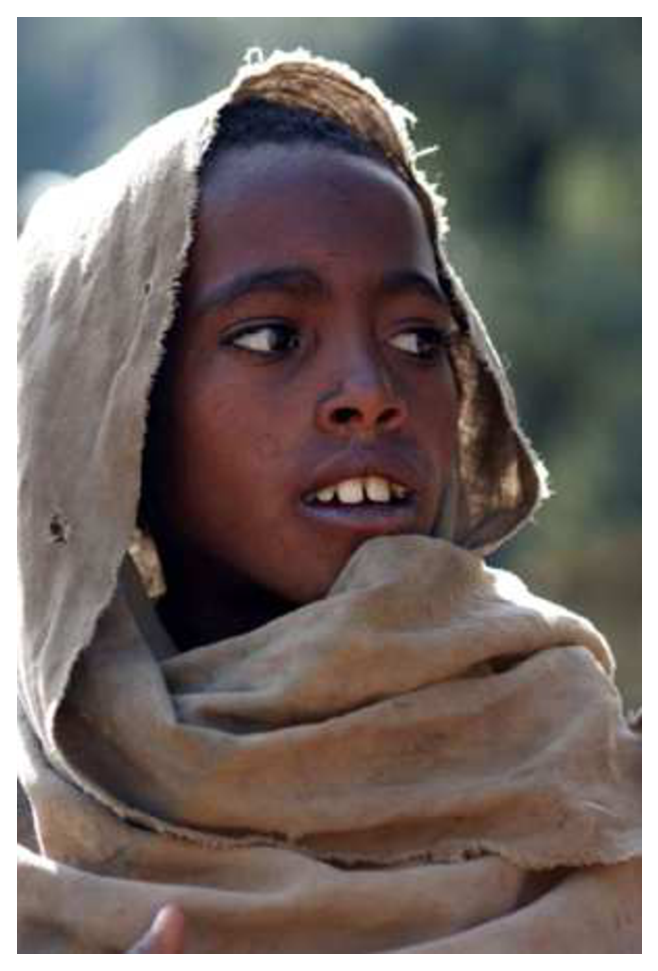
\includegraphics{etiopan.eps}
			\reflectbox{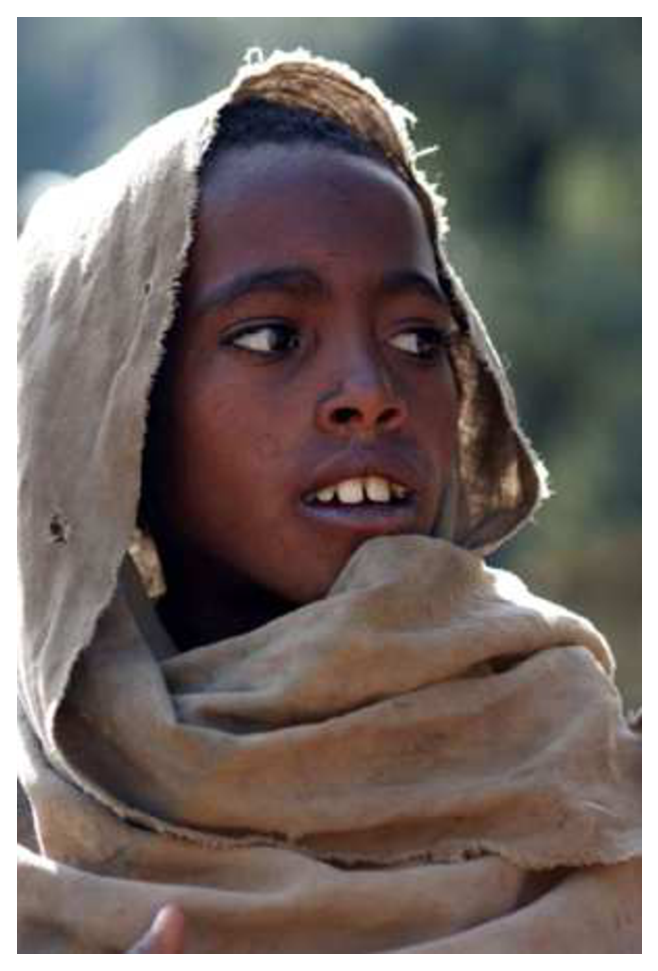
\includegraphics{etiopan.eps}}}
			\caption{Malý Etiopánek a jeho bratříček}
			\label{image1}
		\end{center}
	\end{figure}
	
	\newpage

	Rozdíl mezi vektorovým \dots
	
	\begin{figure}[h]
		\begin{center}
			\scalebox{0.425}{
\includegraphics{oniisan.eps}}
			\caption{Vektorový obrázek}
			\label{image2}
		\end{center}
	\end{figure}

	\dots a bitmapovým obrázkem 
	
	\begin{figure}[h]
		\begin{center}
			\scalebox{0.65}{
\includegraphics{oniisan2.eps}}
			\caption{Bitmapový obrázek}
			\label{image3}
		\end{center}
	\end{figure}

	se projeví například při zvětšení.

	Odkazy (nejen ty) na \ref{image1},  \ref{image2} a  \ref{image3}, na tabulky  \ref{table1}
	a \ref{table2} a také na \ref{alg} jsou udělány pomocí křížových odkazů. Pak je ovšem
	potřeba zdrojový soubor přeložit dvakrát. \\Vektorové obrázky lze vytvořit i přímo v~\LaTeX u, například pomocí prostředí \texttt{picture}.
	
	\newpage
	
	
	\begin{landscape}
	
		\begin{figure}
			\begin{center}
				\begin{picture}(600, 250)
					\put(0,0){\framebox(600, 300){}}
					% line height
					\linethickness{5pt}
					% thick line
					\put(10,50){\line(1,0){580}}
					% line height
					\linethickness{1pt}
					
					\put(80,50){\line(0,1){125}}
					
					\put(80,175){\line(1,0){100}}
					
					\put(140,138){\framebox(405, 20){}}
					\put(180,159){\framebox(150, 30){}}
					\put(331,159){\framebox(180, 5){}}
					
					\put(110,50){\line(0,1){40}}
					\put(110,90){\line(1,0){90}}
					\put(200,90){\line(3,-1){110}}
					\put(245,75){\line(1,0){300}}
					\put(245,75){\line(1,0){300}}
					\put(545,50){\line(0,1){25}}
					
					
					\put(540,75){\line(0,1){47.5}}
					\put(210,87){\line(0,1){35}}
					\put(209.5,122){\line(1,0){330}} 
					
					\put(140,138){\line(5,-6){40}}

					\put(520,240){\circle{80}}

					\end{picture}
				\caption{Vektorový obrázek}
			\end{center}
		\end{figure}
	
	\end{landscape}
\end{document}